So-called open boundary conditions have a special meaning in computational geodynamics. 
They usually refer to the boundary conditions on the sides of Cartesian models, 
usually looking at subduction or rifting processes. 

In the literature boundary conditions on the vertical sidewalls are usually 
\begin{itemize}
\item no-slip (no flow at the boundary), 
\item free slip (impermeable); 
\item open to some particular form of through-flow.
\end{itemize}

Free slip is the most commonly used boundary condition while prescribed in- and outflow 
or periodic boundary conditions are also common. (REF?)

Taken from Chertova et al (2012) \cite{chgv12}:
"Open boundaries for which the horizontal in- and outflow are defined by a fully 
internally developed flow, have hardly been used [...]. 
Such open boundaries basically prescribe a hydrostatic pressure condition on 
the boundary preventing the model to collapse while horizontal in and outflow is free, 
in the sense that it is driven by the internal dynamics and the usual condition of 
incompressible flow. 
Among the range of boundary conditions used, open boundaries may fit best to 
real-mantle flow conditions surrounding subduction zones." 

Two examples of the use of such boundary conditions were found in 
the literature: \cite{qusp10} and \cite{chgv12}.

We start again from the variational form of the momentum equation, and focus on the term containing 
the full stress tensor ${\bm \sigma}$. 
Let us look at the stress tensor gradient, multiplied by the shape function $N$, integrated over the domain:
\begin{eqnarray}
\int_V N {\vec \nabla}\cdot {\bm \sigma} \; dV 
&=&\int_V \left[ {\vec \nabla}\cdot(N {\bm \sigma}) -{\vec \nabla}N \cdot {\bm \sigma}\right] \; dV \nonumber\\
&=& \int_V  {\vec \nabla}\cdot(N {\bm \sigma})\;  dV -\int_V  {\vec \nabla}N \cdot {\bm \sigma} \; dV
\end{eqnarray}
The right term yields the $\K$ and $\G$ matrices after discretisation, as seen in Section~\ref{XXX}.
Turning to the left term, we then make use of the Green-Gauss divergence 
theorem\footnote{\url{https://en.wikipedia.org/wiki/Divergence_theorem}} which states that for 
a continuously differentiable vector field $\vec{F}$:
\[
\int_V ({\vec \nabla} \cdot {\vec F})\; dV = \int _S {\vec F}\cdot {\vec n} \; dS
\]
so that (applying it now to tensors):
\[
\int_V  {\vec \nabla}\cdot(N {\bm \sigma})\;  dV =\int_S  N {\bm \sigma} \cdot {\vec n} \;  dS
\]
This right hand side term is responsible for the surface 
boundary conditions and cannot be neglected if one 
wishes to implement stress boundary conditions, 
such as the so-called open boundary conditions. 

%.................................................................
\subsubsection{two-dimensional case - $Q_1 \times P_0$ elements}

On the following figure two elements are represented, one on the 
left boundary, one on the right boundary:
\begin{center}
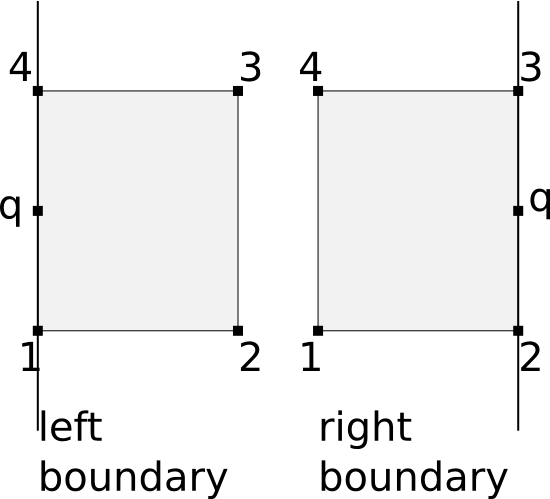
\includegraphics[width=5cm]{images/openbc/drawing.png}
\end{center}

The prescribed traction on the leftt boundary is
\[
{\vec t}={\bm \sigma}\cdot {\vec n}=
\left(
\begin{array}{cc}
-p_{bc} & 0 \\
0 & -p_{bc}
\end{array}
\right)
\cdot
\left(
\begin{array}{c}
-1 \\ 0
\end{array}
\right)
=
\left(
\begin{array}{c}
p_{bc} \\ 0
\end{array}
\right)
\]
The integral on the side of the element is then 
\[
\int_\Gamma N_i {\vec t} \; dS
\]
for $i=1,2,3,4$, which yields the following elementalrhs vector:
\[
\vec{F}=
\int_{\Gamma_{14}} 
\left(
\begin{array}{c}
N_1(x,y) t_x(x,y)\\
N_1(x,y) t_y(x,y)\\
N_2(x,y) t_x(x,y)\\
N_2(x,y) t_y(x,y)\\
N_3(x,y) t_x(x,y)\\
N_3(x,y) t_y(x,y)\\
N_4(x,y) t_x(x,y)\\
N_4(x,y) t_y(x,y)
\end{array}
\right)
\; dS
\]
It is worth noting that the integral takes place on $\Gamma_{14}$ 
so that $N_2$ and $N_3$ are identically zero on this edge
and also $t_y=0$ 
so 
\[
\vec{F}=
\left(
\begin{array}{c}
\int_{\Gamma_{14}}  N_1(x,y) t_x(x,y) dS\\
0 \\
0 \\ 0 \\ 0 \\ 0 \\
\int_{\Gamma_{14}} N_4(x,y) t_x(x,y) dS\\
0
\end{array}
\right)
\]
If the traction (applied pressure) is constant over the element, 
then  
\[
\vec{F}=
t_x
\left(
\begin{array}{c}
\int_{\Gamma_{14}}  N_1(x,y)  dS\\
0 \\
0 \\ 0 \\ 0 \\ 0 \\
\int_{\Gamma_{14}} N_4(x,y)  dS\\
0
\end{array}
\right)
=
t_x
\left(
\begin{array}{c}
\int_{y_1}^{y_4} N_1(x,y) dy\\
0 \\
0 \\ 0 \\ 0 \\ 0 \\
\int_{y_1}^{y_4} N_4(x,y) dy\\
0
\end{array}
\right)
=
\frac{t_x h_y}{2}
\left(
\begin{array}{c}
1 \\
0 \\
0 \\ 0 \\ 0 \\ 0 \\
1 \\
0
\end{array}
\right)
\]
where $h_y$ is the height of the element along the segment. 




Let us recall the elemental vector for the buoyancy term 
${\bm B}_{\rho g}^{el}=\int_\Omega N \rho {\bm g}dV$:
\[
{\bm B}_{el}^{\rho g}(r_q,s_q) =
\left(
\begin{array}{c}
N_1(r_q,s_q) \rho(r_q,s_q) gx\\
N_1(r_q,s_q) \rho(r_q,s_q) gy\\
N_2(r_q,s_q) \rho(r_q,s_q) gx\\
N_2(r_q,s_q) \rho(r_q,s_q) gy\\
N_3(r_q,s_q) \rho(r_q,s_q) gx\\
N_3(r_q,s_q) \rho(r_q,s_q) gy\\
N_4(r_q,s_q) \rho(r_q,s_q) gx\\
N_4(r_q,s_q) \rho(r_q,s_q) gy\\
\end{array}
\right)
\omega_q |J|
\] 
It follows that the corresponding additional elemental right hand side vector writes
for the left open boundary (note that here $r_q,s_q$ are taken on the 1-4 edge):
\[
{\bm B}^{\Gamma,left}_{el}(r_q,s_q) =
h
\left(
\begin{array}{c}
N_1(r_q,s_q) t_x(r_q,s_q) \\
N_1(r_q,s_q) t_y(r_q,s_q) \\
N_2(r_q,s_q) t_x(r_q,s_q) \\
N_2(r_q,s_q) t_y(r_q,s_q) \\
N_3(r_q,s_q) t_x(r_q,s_q) \\
N_3(r_q,s_q) t_y(r_q,s_q) \\
N_4(r_q,s_q) t_x(r_q,s_q) \\
N_4(r_q,s_q) t_y(r_q,s_q) 
\end{array}
\right)
=
(y_4-y_1)
\left(
\begin{array}{c}
-p(r_q,s_q)/2 \\
0\\
0\\
0\\
0\\
0\\
-p(r_q,s_q)/2 \\
0
\end{array}
\right)
\] 
The function $p$ in this case is the pre-computed lithostatic pressure.

And for the right boundary, the corresponding additional elemental right hand side vector writes:

\[
{\bm B}^{\Gamma,right}_{el} =
h
\left(
\begin{array}{c}
N_1(r_q,s_q) t_x(r_q,s_q) \\
N_1(r_q,s_q) t_y(r_q,s_q) \\
N_2(r_q,s_q) t_x(r_q,s_q) \\
N_2(r_q,s_q) t_y(r_q,s_q) \\
N_3(r_q,s_q) t_x(r_q,s_q) \\
N_3(r_q,s_q) t_y(r_q,s_q) \\
N_4(r_q,s_q) t_x(r_q,s_q) \\
N_4(r_q,s_q) t_y(r_q,s_q) 
\end{array}
\right)
=
(y_3-y_2)
\left(
\begin{array}{c}
0\\
0\\
-p(r_q,s_q)/2 \\
0\\
-p(r_q,s_q)/2 \\
0\\
0\\
0
\end{array}
\right)
\] 


\[
{\bm B}_{el} =
{\bm B}_{el}^{\rho g} + 
{\bm B}^{\Gamma,right}_{el} + 
{\bm B}^{\Gamma,left}_{el} 
\]

\subsubsection{three-dimensional case}

\begin{center}
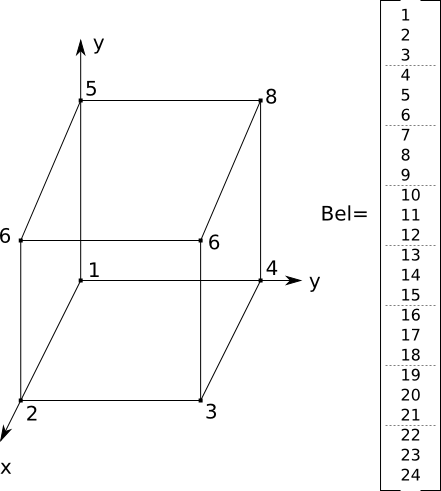
\includegraphics[width=5.5cm]{images/openbc/drawing3D.png}
\end{center}

The face xleft is made of nodes 1,4,5,8, so we need 
to add terms in $B_{el}(1,10,13,22)$. Its surface is 
$S=(y_4-y_1)((z_5-z_1)+(z_8-z_4))/2$, and the lithostatic pressure 
at its center is given by $p=(p_1+p_4+p_5+p_8)/4$.

The face xright is made of nodes 2,3,6,7, so we need 
to add terms in $B_{el}(4,7,16,19)$.

The face yleft is made of nodes 1,2,5,6, so we need 
to add terms in $B_{el}(2,5,14,17)$.

The face xright is made of nodes 3,4,7,8, so we need 
to add terms in $B_{el}(8,11,20,23)$.

%\begin{center}
%\includegraphics[width=4cm]{FEM/openbc/openbc1.png}
%\includegraphics[width=4cm]{FEM/openbc/openbc2.png}\\
%{\small Example of a Stokes sphere sinking when 
%both $y=0$ and $y=L_y$ walls are subjected to
%open boundary conditions.}
%\end{center}



